\clearpage

\begin{usecase}
    \addheading{Use-Case Description}
    \addsingletwocolumnrow{Name}{ugSecurelyUseSystem}
    \addsingletwocolumnrow{Scope}{System}
    \addsingletwocolumnrow{Altitude}{user-goal}
    \addrowheading{Parameters}
    \addnumberedsinglerow{}{none}
    \addrowheading{Primary actor(s)}
    \addnumberedsinglerow{}{\msrcode{actAuthenticated[abstract]}}
    \addrowheading{Secondary actor(s)}
    \addnumberedsinglerow{}{none}
    \addrowheading{Goal(s) description}
    \addsinglerow{the goal is to follow an identification procedure and thus be allowed to safely use the system and it's features.}
    \addrowheading{Reuse}
    \addnumberedsinglerow{}{\msrucname{oeLogin}}
    \addnumberedsinglerow{}{\msrucname{oeLogout}}
    \addrowheading{Protocol condition(s)}
    \addnumberedsinglerow{}{the \msricrash system has been deployed.}
    \addnumberedsinglerow{}{the a useraccount has been created for the user trying to securely use the system.}
    \addrowheading{Pre-condition(s)}
    \addnumberedsinglerow{}{none}
    \addrowheading{Main post-condition(s)}
    \addnumberedsinglerow{}{the \msrcode{actAuthenticated} is known by the system not to be logged.}
    \addrowheading{Main success steps}
    \addalphanumberedsinglerow{}{the actor \msrcode{actAuthenticated} executes the \msrucname{oeLogin} use case.}
    \addalphanumberedsinglerow{}{the actor \msrcode{actAuthenticated} executes the \msrucname{oeLogout} use case}
    \addrowheading{Step Constraints Ordering and Extensions}
    \addnumberedsinglerow{}{step (a) must always precede step (b).}
    \addrowheading{Additional Information}
    \addsinglerow{none.}
\end{usecase}

\clearpage

\begin{figure}[htbp]
\begin{center}
\scalebox{0.95}{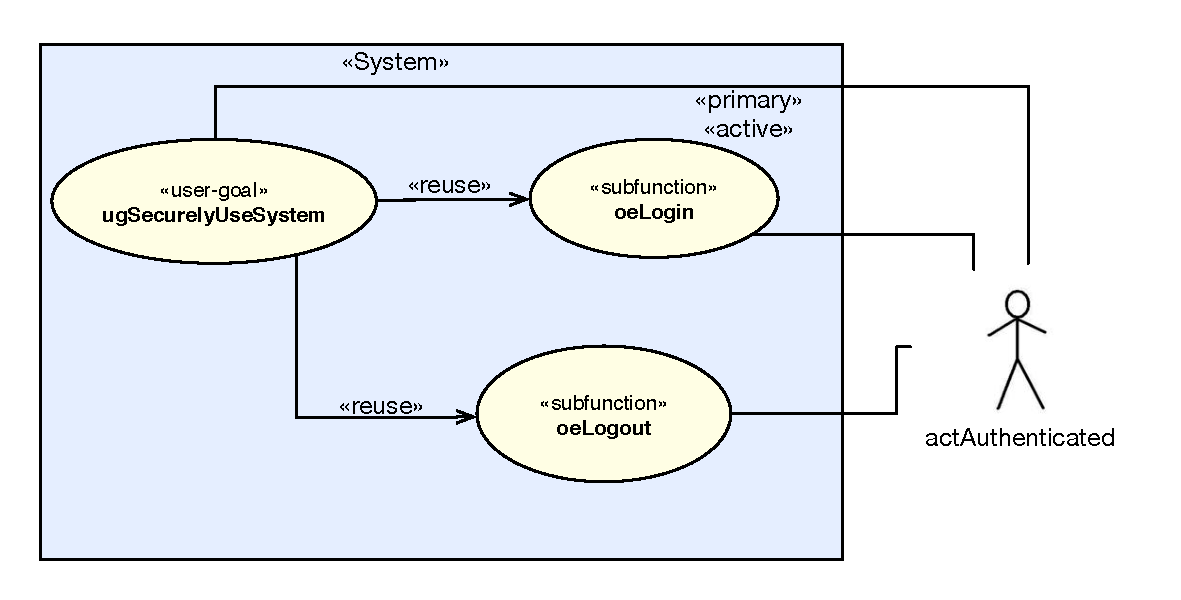
\includegraphics[width=180mm]{./images/ugSecurelyUseSystem.eps}\normalsize}
\end{center}
\caption[\msricrash Use Case Diagram: ugSecurelyUseSystem Diagram]{\msricrash Use Case Diagram: ugSecurelyUseSystem}
\label{fig:icrash-RE-UCD-ugSecurelyUseSystem}
\end{figure}
\vspace{0.5cm}

